% https://tex.stackexchange.com/a/232914/173708
\documentclass[border=9]{standalone}

\usepackage[svgnames, dvipsnames, table]{xcolor}
\definecolor{dgreen}{rgb}{.1,.6,.1}
\definecolor{orchid}{RGB}{218, 112, 214}
\definecolor{brandeisblue}{rgb}{0.0, 0.44, 1.0}
\definecolor{cornflowerblue}{rgb}{0.3921, 0.5843, 0.9294}
\definecolor{limegreen}{rgb}{0.2, 0.8, 0.2}
\definecolor{firebrick}{rgb}{0.7, 0.13, 0.13}

% \usepackage{xspace}
\usepackage{tikz-cd}
\usetikzlibrary{mindmap}

\newcount\tikznumberofcurrentgrandchild

\def\tikzretangulargroth{%
    \pgftransformreset
    \ifnum\tikztreelevel=1
        \pgftransformrotate{30+((\pgfkeysvalueof{/tikz/sibling angle})*(\tikznumberofcurrentchild)}%
        \pgftransformxshift{\the\tikzleveldistance}%
    \fi
    \ifnum\tikztreelevel=2
        \pgfmathsetmacro\tikzoffsetofcurrentchild{(\tikzsiblingdistance)*(\tikznumberofcurrentgrandchild)}%
        \ifdim\tikzoffsetofcurrentchild pt<\tikzlevelwidth pt
            \pgftransformxshift{\tikzlevelwidth/2-\tikzoffsetofcurrentchild}
            \pgftransformyshift{\tikzlevelheight/2}
        \else
        \pgfmathsetmacro\tikzoffsetofcurrentchild{\tikzoffsetofcurrentchild-\tikzlevelwidth}%
        \ifdim\tikzoffsetofcurrentchild pt<\tikzlevelheight pt
            \pgftransformxshift{-\tikzlevelwidth/2}
            \pgftransformyshift{\tikzlevelheight/2-\tikzoffsetofcurrentchild}
        \else
        \pgfmathsetmacro\tikzoffsetofcurrentchild{\tikzoffsetofcurrentchild-\tikzlevelheight}%
        \ifdim\tikzoffsetofcurrentchild pt<\tikzlevelwidth pt
            \pgftransformxshift{-\tikzlevelwidth/2+\tikzoffsetofcurrentchild}
            \pgftransformyshift{-\tikzlevelheight/2}
        \else
        \pgfmathsetmacro\tikzoffsetofcurrentchild{\tikzoffsetofcurrentchild-\tikzlevelwidth}%
        \ifdim\tikzoffsetofcurrentchild pt<\tikzlevelheight pt
            \pgftransformxshift{\tikzlevelwidth/2}
            \pgftransformyshift{-\tikzlevelheight/2+\tikzoffsetofcurrentchild}
        \fi\fi\fi\fi
        \global\advance\tikznumberofcurrentgrandchild by1
    \fi
}
\tikzset{
    branch color/.style={
        concept color=#1!white,
        every child/.append style={concept color=#1!white!30!white},
    },
    level width/.store in=\tikzlevelwidth,
    level height/.store in=\tikzlevelheight
}

\begin{document}
\tikznumberofcurrentgrandchild=0

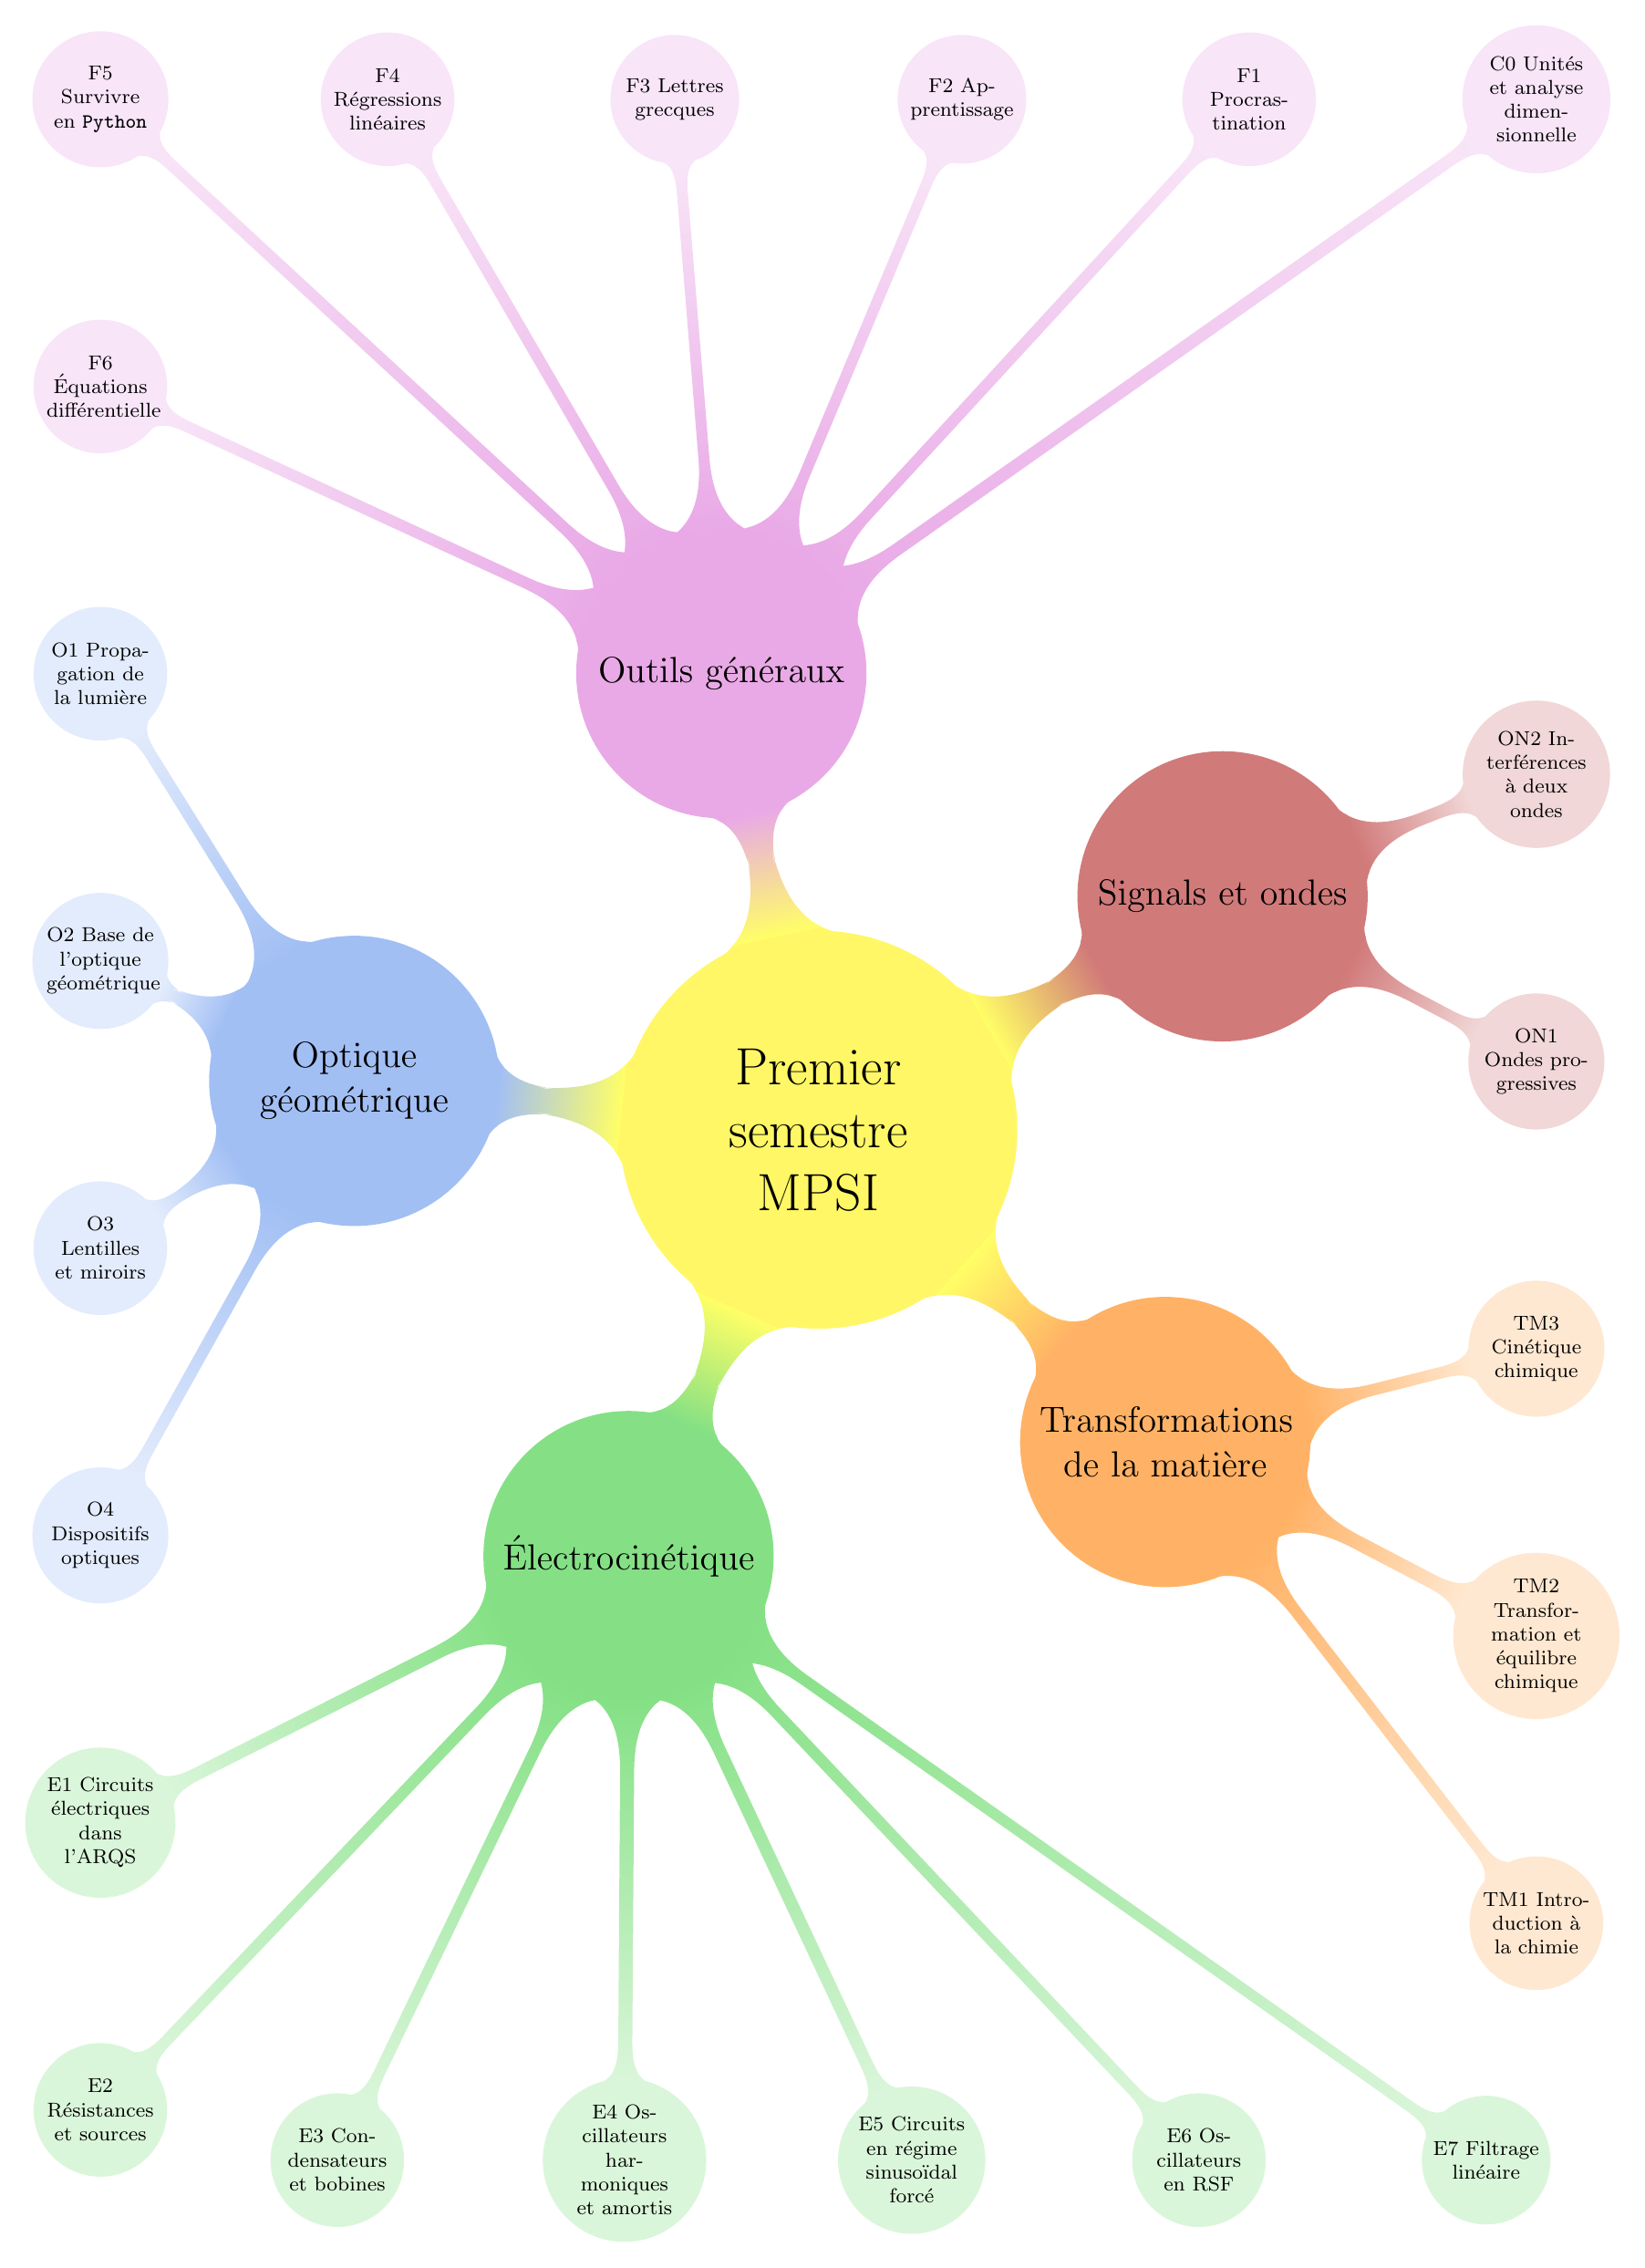
\begin{tikzpicture}[
		mindmap,
		growth function=\tikzretangulargroth,
		nodes={concept},
		concept color=yellow!60,
		root concept/.append style={font=\huge, minimum size=5.5cm},
		level 1/.append style={level distance=6.5cm, sibling angle=360/5},
		level 1 concept/.append style={font=\Large,
				minimum size=4cm, text width=3.5cm},
		level 2/.append style={level width=20cm,level height=28.7cm,
				sibling distance=4cm},
		% A4 paper with margin=.5cm
	]
	\node [root concept]{Premier semestre MPSI}
	child [branch color=orchid!60]{node {Outils généraux}
			child {node {C0 Unités et analyse dimensionnelle}}
			child {node {F1 Procrastination}}
			child {node {F2 Apprentissage}}
			child {node {F3 Lettres grecques}}
			child {node {F4 Régressions linéaires}}
			child {node {F5 Survivre en \texttt{Python}}}
			child {node {F6 Équations différentielles}}
		}
	child [branch color=cornflowerblue!60]{node {Optique géométrique}
			child {node {O1 Propagation de la lumière}}
			child {node {O2 Base de l'optique géométrique}}
			child {node {O3 Lentilles et miroirs}}
			child {node {O4 Dispositifs optiques}}
		}
	child [branch color=limegreen!60]{node {Électrocinétique}
			child {node {E1 Circuits électriques dans l'ARQS}}
			child {node {E2 Résistances et sources}}
			child {node {E3 Condensateurs et bobines}}
			child {node {E4 Oscillateurs harmoniques et amortis}}
			child {node {E5 Circuits en régime sinusoïdal forcé}}
			child {node {E6 Oscillateurs en RSF}}
			child {node {E7 Filtrage linéaire}}
		}
	child [branch color=orange!60]{node {Transformations de la matière}
			child {node {TM1 Introduction à la chimie}}
			child {node {TM2 Transformation et équilibre chimique}}
			child {node {TM3 Cinétique chimique}}
			% child {node {TM4 Réactions acido-basiques}}
			% child {node {TM5 Réactions de précipitation}}
			% child {node {TM6 Réactions d'oxydo-réduction}}
			% child {node {TM7 Diagrammes potentiel-pH}}
		}
	child [branch color=firebrick!60]{node {Signals et ondes}
			child {node {ON1 Ondes progressives}}
			child {node {ON2 Interférences à deux ondes}}
		}
	% child [branch color=green!50]{node {Mécanique}
	% 		child {node {M1 Cinématique du point}}
	% 		child {node {M2 Dynamique du point}}
	% 		child {node {M3 Mouvements courbes}}
	% 		child {node {M4 Approche énergétique du mouvement}}
	% 		child {node {M5 Mouvements de particules chargées}}
	% 		child {node {M6 Moment cinétique du point}}
	% 		child {node {M7 Mouvements à forces centrales}}
	% 		child {node {M8 Mécanique du solide}}
	% 	}
	% child [branch color=teal!60]{node {Architecture de la matière}
	% 		child {node {AM1 Structure des entités chimiques}}
	% 		child {node {AM2 Du micro- au macroscopique}}
	% 		child {node {AM3 Solides cristallins}}
	% 	}
	% child [branch color=yellow!80]{node {Thermodynamique}
	% 		child {node {T1 Description d'un système à l'équilibre}}
	% 		child {node {T2 Premier principe de la thermodynamique}}
	% 		child {node {T3 Second princpe et machines thermiques}}
	% 		child {node {T4 Changements d'états}}
	% 	}
	% child [branch color=green!50]{node {Induction}
	% 		child {node {I1 Champs magnétiques}}
	% 		child {node {I2 Actions mécaniques}}
	% 		child {node {I3 Lois de l'induction}}
	% 		child {node {I4 Conversions électromécaniques}}
	% 	}
	% child [branch color=teal!60]{node {Mécanique quantique}
	% 		child {node {MQ1 Introduction à la mécanique quantique}}
	% 	}
	;
\end{tikzpicture}
\end{document}
